%% LyX 2.4.4 created this file.  For more info, see https://www.lyx.org/.
%% Do not edit unless you really know what you are doing.
\documentclass[english,t]{beamer}
\usepackage{mathptmx}
\usepackage[T1]{fontenc}
\usepackage[latin9]{inputenc}
\usepackage{amssymb}
\usepackage{cancel}

\makeatletter

%%%%%%%%%%%%%%%%%%%%%%%%%%%%%% LyX specific LaTeX commands.
%% Because html converters don't know tabularnewline
\providecommand{\tabularnewline}{\\}

%%%%%%%%%%%%%%%%%%%%%%%%%%%%%% Textclass specific LaTeX commands.
% this default might be overridden by plain title style
\newcommand\makebeamertitle{\frame{\maketitle}}%
% (ERT) argument for the TOC
\AtBeginDocument{%
  \let\origtableofcontents=\tableofcontents
  \def\tableofcontents{\@ifnextchar[{\origtableofcontents}{\gobbletableofcontents}}
  \def\gobbletableofcontents#1{\origtableofcontents}
}

%%%%%%%%%%%%%%%%%%%%%%%%%%%%%% User specified LaTeX commands.
\usetheme{Warsaw}
% or ...

\setbeamercovered{transparent}
% or whatever (possibly just delete it)
\setbeamercovered{invisible} %makes overlays invisible

%gets rid of navigation symbols
\setbeamertemplate{navigation symbols}{}

%\usepackage{hyperref}
%\usepackage[usenames,dvipsnames,table]{xcolor} %adds additional color options
\definecolor{links}{HTML}{2A1B81}
%\hypersetup{colorlinks,linkcolor=blue,urlcolor=links}

\usepackage{multicol}

\usepackage{hyperref}

\usepackage{tikz}
\usetikzlibrary{calc}
\usetikzlibrary{plotmarks}
\usetikzlibrary{shapes}
\usepackage{pgfplots} %\usepackage{pgfplots, pgfplotstable}
\pgfplotsset{compat=newest}
\usepackage{filecontents}  %allows in file data
\usepgfplotslibrary{statistics} %allows histogram stuff

\usepackage{forest} %%for tree diagram

\usepackage{calc}
\usepackage[nomessages]{fp}

\usepackage[super]{nth} %easy 1st, 2nd, etc

%\usepackage{advdate}    % Advancing/saving dates
\usepackage{datetime}   % Dates formatting
%\usepackage{datenumber} % Counters for dates

\usepackage[super]{nth}

\usepackage{etex}

\usepackage{fancybox}

%%table colors
%\usepackage[table]{xcolor}
\usepackage{colortbl}

\usepackage[outline]{contour}  %allows text halos

\usepackage{epsdice} %%dice font
\usepackage[misc]{ifsym}
\newfont\dice{dice3d} %%3d dice font

\contourlength{1pt} %sets halo width
%%example: \node at (0.75,0.5) {\contour{white}{\Large Text!}};
%%example:  \node [fill=white,inner sep=1pt] at (2.25,0.5) {\Large 			Text!};
%%example:  \node [fill=white,rounded corners=2pt,inner sep=1pt] at 			(3.75,0.5) {\Large Text!};

%%%%%%%%%%%%%%%%%%%%%%%%%%%
\def\formatdateny{\csname noyear\languagename\expandafter\endcsname\formatdate}
\def\noyearenglish#1, \the\@year{#1}
\let\noyearamerican\noyearenglish
\let\noyearbritish\noyearenglish

%%allows uncover with forest diagrams
\tikzset{
    invisible/.style={opacity=0,text opacity=0},
    visible on/.style={alt=#1{}{invisible}},
    alt/.code args={<#1>#2#3}{%
      \alt<#1>{\pgfkeysalso{#2}}{\pgfkeysalso{#3}} % \pgfkeysalso doesn't change the path
    },
}
\forestset{
  visible on/.style={
    for tree={
      /tikz/visible on={#1},
      edge={/tikz/visible on={#1}}}}}

%%%redefines column alignment to match vertically
%\define@key{beamerframe}{t}[true]{% top
  %\beamer@frametopskip=.2cm plus .5\paperheight\relax%
  %\beamer@framebottomskip=0pt plus 1fill\relax%
 % \beamer@frametopskipautobreak=\beamer@frametopskip\relax%
  %\beamer@framebottomskipautobreak=\beamer@framebottomskip\relax%
  %\def\beamer@initfirstlineunskip{}%
%}

%%provides pdf with 4 slides per page; don't forget to add 'handout' to remove overlays
%\usepackage{pgfpages}
%\pgfpagesuselayout{4 on 1}[a4paper, landscape, border shrink=7mm]
%\pgfpageslogicalpageoptions{1}{border code=\pgfusepath{stroke}}
%\pgfpageslogicalpageoptions{2}{border code=\pgfusepath{stroke}}
%\pgfpageslogicalpageoptions{3}{border code=\pgfusepath{stroke}}
%\pgfpageslogicalpageoptions{4}{border code=\pgfusepath{stroke}}
%%%Don't forget to add 'handout'

\makeatother

\usepackage{babel}
\begin{document}
%%data for exams%%
\begin{filecontents}{exam_data.csv} 
dist 
55 
55 
55 
55 
55 
65 
65 
65 
65 
65 
65 
65 
65 
65 
65 
65 
65 
65 
75 
75 
75 
75 
75 
75 
75 
75 
75 
75 
75 
75 
75
75
75
75
75
75
75
75
75
75
75
75 
75 
75
75 
75 
75 
75
75
75 
75 
75 
75 
75 
75 
75 
75 
75 
75 
75 
75 
75 
75 
75 
75 
75 
75 
75 
75 
75 
75 
75 
75 
75 
75 
75
75 
75 
75 
75 
75 
75 
75 
75 
75 
75 
85 
85 
85 
85 
85 
85 
85 
85 
85 
85 
85 
85 
85 
95 
95 
95   
\end{filecontents}

\newcommand{\xmax}{2000}
\newcommand{\xmin}{0}
\newcommand{\xstep}{0} %must be xmin+n
\newcommand{\ymax}{500}
\newcommand{\ymin}{0}
\newcommand{\ystep}{0} %must be ymin+n

\newcounter{countEx} \setcounter{countEx}{0}
\newcounter{countProb} \setcounter{countProb}{0}
\resetcounteronoverlays{countEx} \resetcounteronoverlays{countProb}

\newcommand{\ex}[3]{
	\addtocounter{countEx}{1}
	\only<#1-#2>{\begin{exampleblock} {Example \chNum.\secNum.\arabic{countEx}.} #3	\end{exampleblock}}
}

\newcommand{\prob}[4]{
	\addtocounter{countProb}{1}
	\only<#1-#2>{\begin{exampleblock} {Problem  \chNum.\secNum.\arabic{countProb}.\,#3} #4	\end{exampleblock}}
}

\newcommand{\yline}[4]{
	(#2 - #4)/(#1 - #3)*(x - #1) + #2
}

\beamerdefaultoverlayspecification{<+->}

%%%%Chapter and Section numbers%%%%%
\newcommand{\chNum}{4}
\newcommand{\secNum}{3}
\newcommand{\secTitle}{Measures of Dispersion}
\date{\formatdate{31}{10}{2014}}

\title[Section \chNum.\secNum: \secTitle]{Section \chNum.\secNum: \secTitle}

\subtitle{Finite Mathematics~~MTH 107~~Fall 2014}

\author{Dr.\,James Ashe}

\titlegraphic{\includegraphics[height=2.75cm]{/home/jim/JamesAshe/MHU/images/MarsHilUniversityLogo-Virtical.png}}

\institute{Mars Hill University}

\makebeamertitle 

%%True false command
\newcommand{\T}{\textcolor{green}{\contour{black}{T}}}
\newcommand{\F}{\textcolor{red}{\contour{black}{F}}}
\newcommand{\uT}[2]{\uncover<#1-#2>{\T}}
\newcommand{\uF}[2]{\uncover<#1-#2>{\F}}

%tkiz ball item 
\newcommand*\circled[1]{\tikz[baseline=(char.base)]
	{\node[circle,ball color=green!50!black!100, shade,   color=white,inner sep=1.2pt] (char) {\tiny #1};
	}
}
\begin{frame}{Dispersion}

\begin{center}
\begin{tabular}{|c|c|c|c|c|c|c|}
\hline 
\cellcolor{yellow!50}\textbf{Munson} & 185 & 135 & 200 & 185 & 250 & 155\tabularnewline
\hline 
\hline 
\cellcolor{yellow!50}\textbf{McCracken} & 182 & 185 & 188 & 185 & 180 & 190\tabularnewline
\hline 
\end{tabular}
\par\end{center}
\begin{columns}


\column{5.5cm}
\begin{itemize}
\item []\textbf{Munson}
\item <2->[]135 155 185 185 200 250
\item <3->[$\bar{x}$]Mean: $\frac{135+155+185+185+200+250}{6}$$=185$
\item <4->[]Median: $\dfrac{185+185}{2}=185$
\item <5->[]Mode: $185$
\end{itemize}

\column{5.5cm}
\begin{itemize}
\item []\textbf{McCracken}
\item <6->[]180 182 185 185 188 190
\item <7->[$\bar{x}$]Mean: $\frac{180+182+185+185+188+190}{6}$$=185$
\item <8->[]Median: $\dfrac{185+185}{2}=185$
\item <9->[]Mode: $185$
\end{itemize}
\end{columns}
\end{frame}

\begin{frame}{Dispersion}

\begin{center}
\begin{tabular}{|c|c|c|c|c|c|c|}
\hline 
\cellcolor{yellow!50}\textbf{Munson} & 185 & 135 & 200 & 185 & 250 & 155\tabularnewline
\hline 
\hline 
\cellcolor{yellow!50}\textbf{McCracken} & 182 & 185 & 188 & 185 & 180 & 190\tabularnewline
\hline 
\end{tabular}
\par\end{center}
\begin{columns}


\column{5.5cm}
\begin{itemize}
\item [] \vfill\textbf{Munson}
\item <2->[]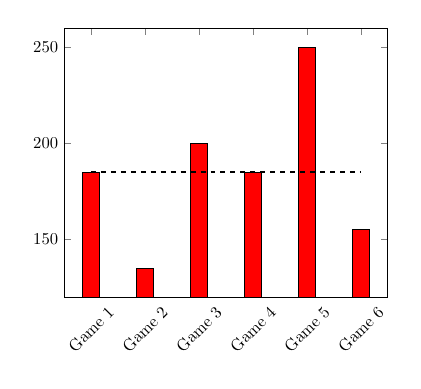
\begin{tikzpicture}[scale=.6]         
	\begin{axis}[             
		symbolic x coords={Game 1, Game 2, Game 3, Game 4, Game 5, Game 6},             
		xtick=data,
		xticklabel style={rotate=45},
		ymin=120,
		ymax=260        
	]             
		\addplot[ybar,fill=red] coordinates {
			(Game 1,   185)
			(Game 2,   135) 
			(Game 3,   200)
			(Game 4,   185)
			(Game 5,   250)
			(Game 6,   155)         
		};
		\draw[black, very thick, dashed] (axis cs:Game 1,185) -- (axis cs:Game 6,185);        
	\end{axis}     
\end{tikzpicture}
\item [] \vfill
\end{itemize}

\column{5.5cm}
\begin{itemize}
\item [] \vspace{-.2cm}\textbf{McCracken}
\item <3->[]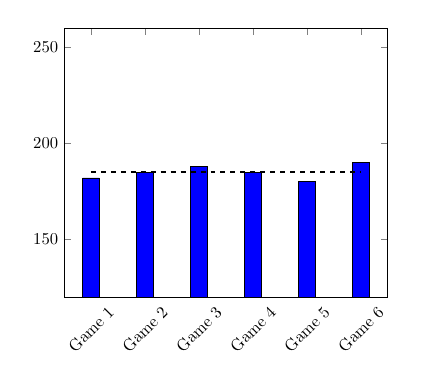
\begin{tikzpicture}[scale=.6]         
	\begin{axis}[             
		symbolic x coords={Game 1, Game 2, Game 3, Game 4, Game 5, Game 6},             
		xtick=data,
		xticklabel style={rotate=45},
		ymin=120,
		ymax=260        
	]             
		\addplot[ybar,fill=blue] coordinates {
			(Game 1,   182)
			(Game 2,   185) 
			(Game 3,   188)
			(Game 4,   185)
			(Game 5,   180)
			(Game 6,   190)         
		};
		\draw[black, very thick, dashed] (axis cs:Game 1,185) -- (axis cs:Game 6,185);         
	\end{axis}     
\end{tikzpicture}
\item [] \vfill
\end{itemize}
\end{columns}
\end{frame}

\begin{frame}{Dispersion}

\begin{center}
\begin{tabular}{|c|c|c|c|c|c|c|}
\hline 
\cellcolor{yellow!50}\textbf{Munson} & 185 & 135 & 200 & 185 & 250 & 155\tabularnewline
\hline 
\multicolumn{1}{c}{\textbf{Deviation: }$x-\bar{x}$} & \multicolumn{1}{c}{$0$} & \multicolumn{1}{c}{$-50$} & \multicolumn{1}{c}{$15$} & \multicolumn{1}{c}{$0$} & \multicolumn{1}{c}{$65$} & \multicolumn{1}{c}{$-30$}\tabularnewline
\hline 
\cellcolor{yellow!50}\textbf{McCracken} & 182 & 185 & 188 & 185 & 180 & 190\tabularnewline
\hline 
\multicolumn{1}{c}{\textbf{Deviation: }$x-\bar{x}$} & \multicolumn{1}{c}{$-3$} & \multicolumn{1}{c}{$0$} & \multicolumn{1}{c}{$3$} & \multicolumn{1}{c}{$0$} & \multicolumn{1}{c}{$-5$} & \multicolumn{1}{c}{$5$}\tabularnewline
\end{tabular}
\par\end{center}
\begin{columns}


\column{5.5cm}
\begin{itemize}
\item [] \vfill\textbf{Munson}
\item <2->[]The ``average'' deviation
\item <3->[]$\frac{0-50+15+0+65-30}{6}$
\item <4->[]$=\frac{0}{6}=0$
\end{itemize}

\column{5.5cm}
\begin{itemize}
\item [] \vspace{-.2cm}\textbf{McCracken}
\item <5->[]The ``average'' deviation
\item <6->[]$\frac{-3+0+3+0-5+5}{6}$
\item <7->[]$=\frac{0}{6}=0$
\end{itemize}
\end{columns}
\begin{itemize}
\item []<8-> NOT the measurement of dispersion we need.

\begin{itemize}
\item []<9->(This always happens!)
\end{itemize}
\end{itemize}
\end{frame}

\begin{frame}{Variance and Standard DeviationDispersion}

\begin{columns}


\column{5.5cm}
\begin{block}{Sample Variance Deviation Given a sample of $n$ data points, $x_{1}$,
$x_{2},\dots,$ $x_{n}$, the \textbf{variance}, $s^{2}$, of the
data is \\
$s^{2}=\dfrac{\sum(x-\bar{x})^{2}}{n-1}$ }
\end{block}

\begin{block}<6->{Standard Devation}
Given a sample of $n$ data points, $x_{1}$, $x_{2},\dots,$ $x_{n}$,
the \textbf{standard deviation}, $s$, of the data is \\
$s=\sqrt{\mbox{variance}}$ 
\end{block}

\column{5.5cm}
\begin{itemize}
\item <2->[]\textbf{Variance}

\begin{itemize}
\item <3->[]Data is almost always a sample.
\item <4->[]Population will vary more than a sample, so $n-1$ is used
so the variance will not be underestimated.
\item <5->[]\emph{Bessel's correction}
\end{itemize}
\item <6->[]\textbf{Standard Deviation}

\begin{itemize}
\item <7->[]The ``average'' distance from the mean.
\end{itemize}
\end{itemize}
\end{columns}
\end{frame}

\begin{frame}{Variance and Standard DeviationDispersion}

\vspace{-.5cm}
\begin{columns}


\column{5.5cm}
\begin{block}{Sample Variance Deviation Given a sample of $n$ data points, $x_{1}$,
$x_{2},\dots,$ $x_{n}$, the \textbf{variance}, $s^{2}$, of the
data is \\
$s^{2}=\dfrac{\sum(x-\bar{x})^{2}}{n-1}$ }
\end{block}

\column{5.5cm}
\begin{block}{Standard DevationGiven a sample of $n$ data points, $x_{1}$, $x_{2},\dots,$
$x_{n}$, the \textbf{standard deviation}, $s$, of the data is \\
$s=\sqrt{\mbox{variance}}$}
\end{block}
\end{columns}
\begin{center}
\begin{tabular}{ccccccc}
\hline 
\multicolumn{1}{|c|}{\cellcolor{yellow!50}\textbf{Munson}} & \multicolumn{1}{c|}{185} & \multicolumn{1}{c|}{135} & \multicolumn{1}{c|}{200} & \multicolumn{1}{c|}{185} & \multicolumn{1}{c|}{250} & \multicolumn{1}{c|}{155}\tabularnewline
\hline 
\textbf{ }$x-\bar{x}$ & $0$ & $-50$ & $15$ & $0$ & $65$ & $-30$\tabularnewline
\uncover<2->{$(x-\bar{x)^{2}}$} & \uncover<3->{$0^{2}$} & \uncover<4->{$(-50)^{2}$} & \uncover<5->{$15^{2}$} & \uncover<6->{$0^{2}$} & \uncover<7->{$65^{2}$} & \uncover<8->{$(-30)^{2}$}\tabularnewline
 & \uncover<9->{$0$} & \uncover<9->{$2500$} & \uncover<10->{$225$} & \uncover<10->{$0$} & \uncover<10->{$4225$} & \uncover<10->{$900$}\tabularnewline
\end{tabular}
\par\end{center}
\begin{itemize}
\item <11->[]Sum: $0+2500+225+0+4225+900=7850$
\item <12->[]$s^{2}=\dfrac{7850}{n-1}$\uncover<13->{ $=\dfrac{7850}{5}=1570$}
\item <14->[] $s=\sqrt{1570}$\uncover<15->{ $\approx39.623\dots$}
\end{itemize}
\end{frame}

\begin{frame}{Variance and Standard DeviationDispersion}

\vspace{-.5cm}

\begin{center}
\begin{tabular}{|c|c|c|c|c|c|c|}
\hline 
\cellcolor{yellow!50}\textbf{Munson} & 185 & 135 & 200 & 185 & 250 & 155\tabularnewline
\hline 
\end{tabular}
\par\end{center}
\begin{itemize}
\item [] $s=\sqrt{1570}$$\approx39.623\dots$
\end{itemize}
\begin{center}
\begin{tabular}{ccccccc}
\hline 
\multicolumn{1}{|c|}{\cellcolor{yellow!50}\textbf{McCracken}} & \multicolumn{1}{c|}{182} & \multicolumn{1}{c|}{185} & \multicolumn{1}{c|}{188} & \multicolumn{1}{c|}{185} & \multicolumn{1}{c|}{180} & \multicolumn{1}{c|}{190}\tabularnewline
\hline 
\textbf{ }$x-\bar{x}$ & $-3$ & $0$ & $3$ & $0$ & $-5$ & $5$\tabularnewline
\uncover<2->{$(x-\bar{x)^{2}}$} & \uncover<3->{$(-3)^{2}$} & \uncover<4->{$0^{2}$} & \uncover<5->{$3^{2}$} & \uncover<6->{$0^{2}$} & \uncover<7->{$(-5)$} & \uncover<8->{$5^{2}$}\tabularnewline
 & \uncover<9->{$9$} & \uncover<9->{$0$} & \uncover<10->{$9$} & \uncover<10->{$0$} & \uncover<10->{$25$} & \uncover<10->{$25$}\tabularnewline
\end{tabular}
\par\end{center}
\begin{itemize}
\item <11->[]Sum: $9+0+9+0+25+25=68$
\item <12->[]$s^{2}=\dfrac{68}{n-1}$\uncover<13->{ $=\dfrac{68}{5}=13.6$}
\item <14->[] $s=\sqrt{13.6}$\uncover<15->{ $\approx3.687\dots$}
\end{itemize}
\end{frame}

\begin{frame}{Standard Deviation of Grouped Data}

\begin{tabular}{|c|c|c|c|c|}
\hline 
\rowcolor{yellow!50}\textbf{Grade} & \tiny\uncover<2->{\textbf{Midpoint}} & \textbf{Freq.} & \uncover<4->{$f\cdot x$} & \uncover<8->{$f\cdot x^{2}$}\tabularnewline
\hline 
$50\leq x<60$ & \uncover<3->{$55$} & 3 & \uncover<5->{$165$} & \uncover<9->{$9075$}\tabularnewline
\hline 
$60\leq x<70$ & \uncover<3->{$65$} & 13 & \uncover<6->{$845$} & \uncover<10->{$54925$}\tabularnewline
\hline 
$70\leq x<80$ & \uncover<3->{$75$} & 68 & \uncover<6->{$5100$} & \uncover<11->{$382500$}\tabularnewline
\hline 
$80\leq x<90$ & \uncover<3->{$85$} & 13 & \uncover<6->{$1105$} & \uncover<11->{$93925$}\tabularnewline
\hline 
$90\leq x<100$ & \uncover<3->{$95$} & 3 & \uncover<6->{$285$} & \uncover<11->{$27075$}\tabularnewline
\hline 
\multicolumn{1}{c}{} &  & $n=100$ & \uncover<7->{$\sum f\cdot x=$} & \uncover<12->{$\sum f\cdot x^{2}=$}\tabularnewline
\cline{3-5}
\multicolumn{1}{c}{} &  &  & \uncover<7->{$7500$} & \uncover<12->{$567500$}\tabularnewline
\cline{3-5}
\end{tabular}
\begin{columns}


\column{5.5cm}

\only<1-12>{
\begin{block}{Alt. Formula for Variance$s^{2}=\dfrac{1}{n-1}\left(\sum x^{2}-\dfrac{(\sum x)^{2}}{n}\right)$}
\end{block}
}

\only<13->{
\begin{block}{Alt. Formula for Variance: Grouped data$s^{2}=\dfrac{1}{n-1}\left(\sum f\cdot x^{2}-\dfrac{(\sum f\cdot x)^{2}}{n}\right)$}
\end{block}
}

\column{5.5cm}
\begin{itemize}
\item []<14->$s^{2}=\dfrac{1}{99}\left(567500-\dfrac{(7500)^{2}}{100}\right)$

\begin{itemize}
\item []<14->\textrm{$\approx50.5051$}
\end{itemize}
\item []<15->$s=\sqrt{50.5051}\approx7.1067$
\end{itemize}
\end{columns}
\end{frame}

\begin{frame}{Distributions}

\begin{center}
\begin{tikzpicture}[scale=1.25]
\begin{axis}[     ybar,     ymin=0 ] 
\addplot +[hist={bins=5,data min=50,data max=100}] table [y index=0] {exam_data.csv}; 
\end{axis} 
\end{tikzpicture} 
\par\end{center}
\end{frame}

\end{document}
